%!TEX program = xelatex
\documentclass[format=draft,language=chinese,category=academic-report]{hustreport}
\usepackage{booktabs}
\usepackage{flowchart}
\usetikzlibrary{arrows}
\usepackage[section]{placeins}

% =============================== %

\stuno{U201814468}
\title{数据结构实验}
\author{王清雨}
\major{计卓1801}
\department{计算机科学与技术学院}
\advisor{许贵平\hspace{1em}副教授}

\begin{document}

\frontmatter
\maketitle
%\makeabstract
\tableofcontents

\mainmatter

\chapter{引言}\label{ch:background}

% 选题背景:说明课程设计课题的目的与意义、应解决的主要问题及应达到的技术要求;
% 简述研究与发展概况及存在的问题,本设计的指导思想
\section{课题背景与意义}\label{sec:purpose}

\subsection{课题背景}
编译器(Compiler)是一种计算机程序,它会将某种编程语言写成的源代码(原始语言)
转换成另一种编程语言(目标语言)。
它主要的目的是将便于人编写、阅读、维护的高级计算机语言所写作的源代码程序,
翻译为计算机能解读、运行的低阶机器语言的程序,也就是可执行文件。

编译器将原始程序(Source program)作为输入,翻译产生使用目标语言(Target language)的等价程序。
源代码一般为高级语言(High-level language),如Pascal、C、C++、Java等,
而目标语言则是汇编语言或目标机器的目标代码(Object code),有时也称作机器代码(Machine code)。

早期的计算机软件都是用汇编语言直接编写的,这种状况持续了数年。
当人们发现为不同类型的中央处理器(CPU)编写可重用软件的开销要明显高于编写编译器时,
人们发明了高级编程语言。由于早期的计算机的内存很少,当大家实现编译器时,遇到了许多技术难题。

逐渐地,编译技术成熟了起来,高级语言在许多领域流行也起来。由于新的编程语言支持的功能越来越多,
计算机的架构越来越复杂,这使得编译器也越来越复杂。

早期的编译器是用汇编语言编写的。
首个能编译自己源程序的编译器是在1962年由麻省理工学院的Hart和Levin制作的。
从20世纪70年代起,实现能编译自己源程序的编译器变得越来越可行,
不过还是用Pascal和C语言来实现编译器更加流行。

\autoref{fig:compiler_process}中给出了一个现代编译器完整的工作流程。
其中,本次课题主要研究的是其中{\bf 编译器}的部分,也即俗称的编译器的{\bf 前端}。
主要实现了{\bf 词法分析}和{\bf 语法分析}。

\begin{figure}[hbt]
	\centering
\begin{tikzpicture}[font={\sf \small}]
	\def\smbwd{2cm}

	\node (terminal1) at (0,0) [draw, terminal,
	minimum width=\smbwd,
	minimum height=0.5cm] {源代码};

	\node (predproc1) at (0,-1.5) [draw, storage, align=left,
	minimum width=\smbwd,
	minimum height=1cm] {预处理器};

	\node (decide1) at (0,-3.5) [draw, decision,
  minimum width=\smbwd,
  minimum height=1cm] {编译器};

  \node (storage1) at (0,-5.5) [draw, storage,
  minimum width=\smbwd,
  minimum height=1cm] {汇编程序};

  \node (process1) at (0,-7.25) [draw, storage,
  minimum width=\smbwd,
  minimum height=1cm] {目标代码};

  \node (terminal2) at (0,-9.0) [draw, storage,
  minimum width=\smbwd,
  minimum height=1cm] {链接器};

  \node (terminal3) at (0,-10.5) [draw, terminal,
  minimum width=\smbwd,
  minimum height=0.5cm] {可执行文件};

  \draw[->] (terminal1) -- (predproc1);
  \draw[->] (predproc1) -- (decide1);
  \draw[->] (decide1) --  (storage1);
  \draw[->] (storage1) -- (process1);
  \draw[->] (process1) -- (terminal2);
  \draw[->] (terminal2) -- (terminal3);
\end{tikzpicture}
\caption{现代编译器工作主要流程}\label{fig:compiler_process}
\end{figure}

\subsection{课题意义}

由于高级语言根据程序员的需求变得越来越复杂,因此编译器也随之变得越来越复杂。
著名开源编译器项目LLVM的前端Clang源代码就多达336MB。\footnote{共包含源文件15034个,共有代码1756797行}
其中用到的数据结构数不胜数,各种优化方法也是层出不穷。可以说,对编译器对研究是计算机科学
中最为重要的一个研究领域,可谓皇冠上的明珠。

\section{国内外研究现状}

 众多的编译算法,包括词法分析、类型检查和推导、数据流分析、基于数据依赖性分析的循环变换、
 基于图着色的寄存器分配以及软件流水等,都是计算机科学中的奇葩。
 通过集成到各种功能强大而应用广泛的工具中,这些方法极大地影响着计算领域的实践。
 与早期的编译器实现相比,今天的编译算法明显变得越来越复杂。

 受益于基于自动机理论的词法和语法分析技术的系统化理论的发展,编译器的前端有了更加
 系统化、自动化的开发方式。因此,目前对于编译器的研究重点不再是如何实现,
 而是在于{\bf 性能}与{\bf 安全性}的提升。\cite{Advanced-compiler-optim,53e9b0b2b7602d9703b20db9}

\section{课程设计的主要研究工作}

\subsection{任务提炼}

正如\autoref{sec:purpose}所述,本次任务的主要目的是实现一个编译器的前端。
因此,我将本次任务分为以下几个步骤:

\begin{enumerate}
  \item 根据给出的要求,使用巴克斯(BNF)范式定义高级语言的词法规则、语法规则。
  \item 根据定义的词法规则,编写词法分析器。
  \item 根据定义的语法规则,编写语法分析器。
  \item 对编译器进行性能上的优化。
  \item 对编译器进行完善的测试(包括正确性测试以及错误处理测试)。
  \item 总结整个任务的完成情况,并展望未来可以提高的方面。
\end{enumerate}

\subsection{任务分析}

\paragraph{定义语言的巴克斯范式}

巴克斯范式是一种用于表示上下文无关文法的语言,上下文无关文法描述了一类形式语言,
它更广泛地使用于程序设计语言、指令集、通信协议的语法表示中。
通过巴克斯范式,我们能够精确、直观地定义语言的组成部分
(例如:{\it 标识符、数字、关键字、语句构成等})。
从而才能编写词法分析器与语法分析器,因此我们首先需要严格规定我们编译器所针对的语言,
才能更好的进行接下来的步骤。

\paragraph{词法分析}

词法分析部分是整个任务的基础,也是编译器能识别源文件的关键。词法分析通过有限自动状态机
(FSA)进行分词(tokenize),将源文件(视为文本)根据空格、换行等分隔符划分为
一个个词(token)。\autoref{fig:lex_FSM}中给出了有限自动状态机的部分定义
(没有包括全部关键词和运算符)。

\begin{figure}[hbt]
  \centering
  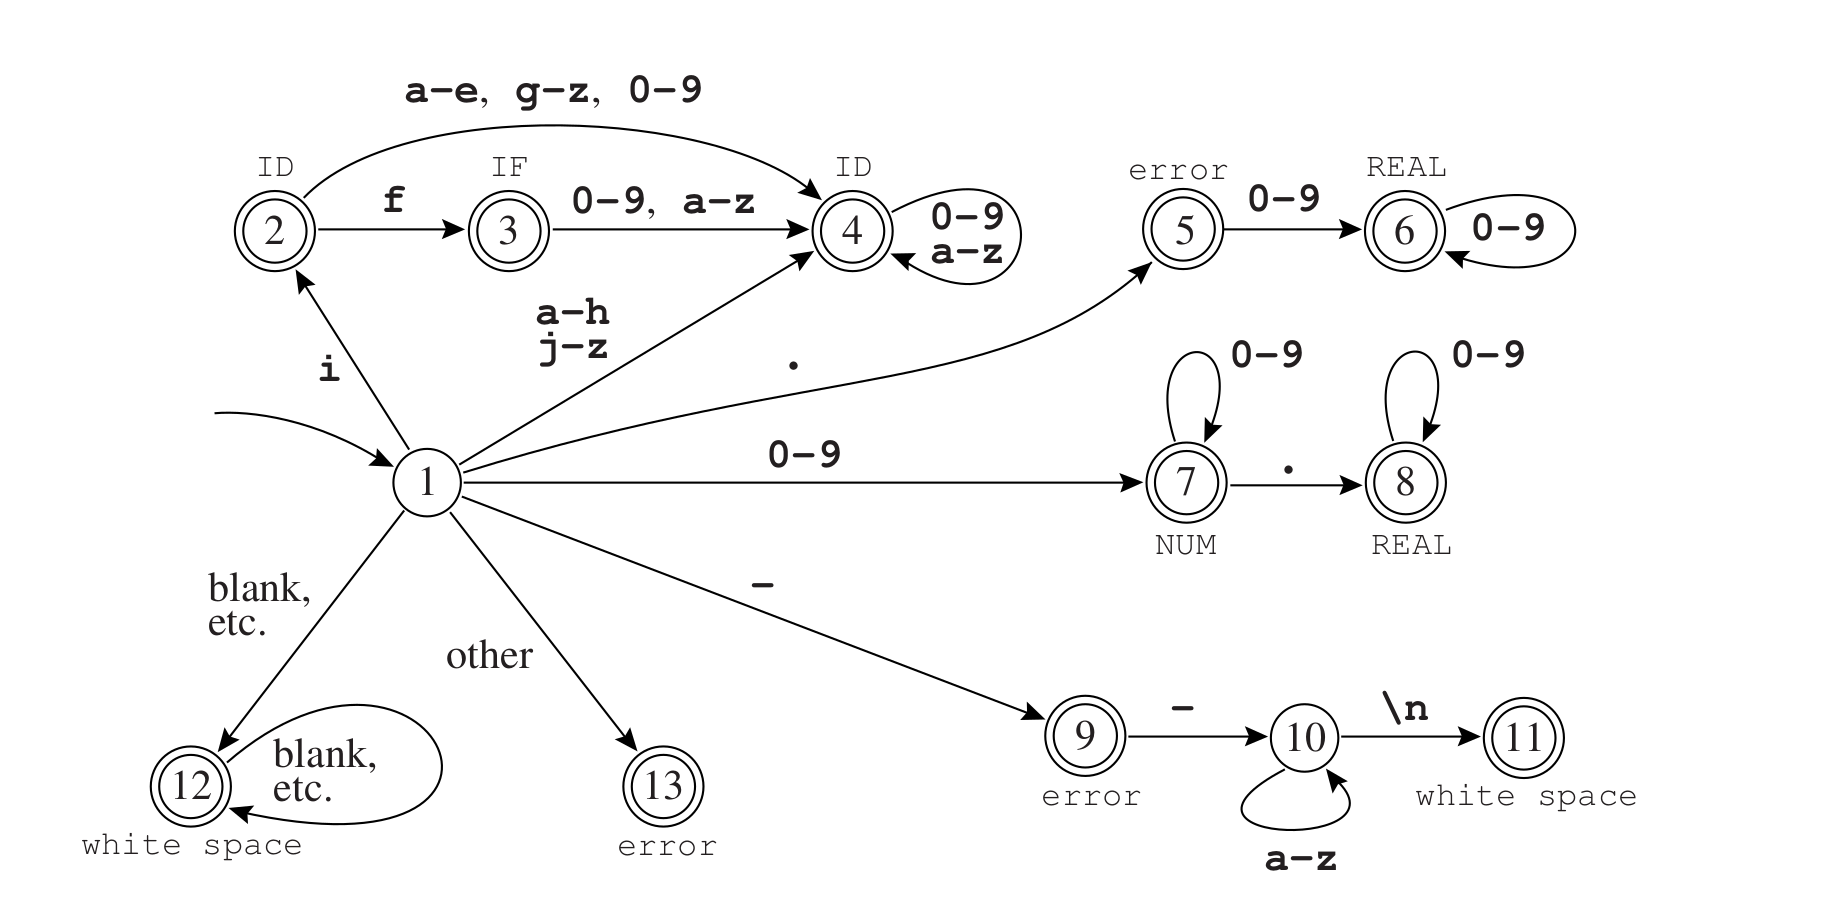
\includegraphics[scale=.25]{FSM1.png}
  \caption{词法分析有限自动状态机}\label{fig:lex_FSM}
\end{figure}

\paragraph{语法分析}

经过了词法分析后,编译器已经能够识别源文件中每一个语素是什么了,但是还不清楚它们组合起来是什么意思。
于是我们就要进行语法分析,根据定义的巴克斯范式,分析我们的语素是否组合正确。
在本次任务中,我选择使用较为简单的递归下降(Recursive descent)算法来进行词法分析。
\cite{53e9b0b2b7602d9703b20db9,Recursive-programming,appel2004modern,muchnick1997advanced,aho1986compilers}

递归下降算法是一种自顶向下的解析器,用于解析LL语法\cite{aho1986compilers}。
需要编写一组相互递归调用的过程,其中每个过程都实现了一部分都语法内容。
最终语法分析器的结构会与所定义的语法紧密相连。
\autoref{fig:recursive-decent}给出了一个简单的递归下降生成语法树的例子。

\begin{figure}[hbt]
  \centering
  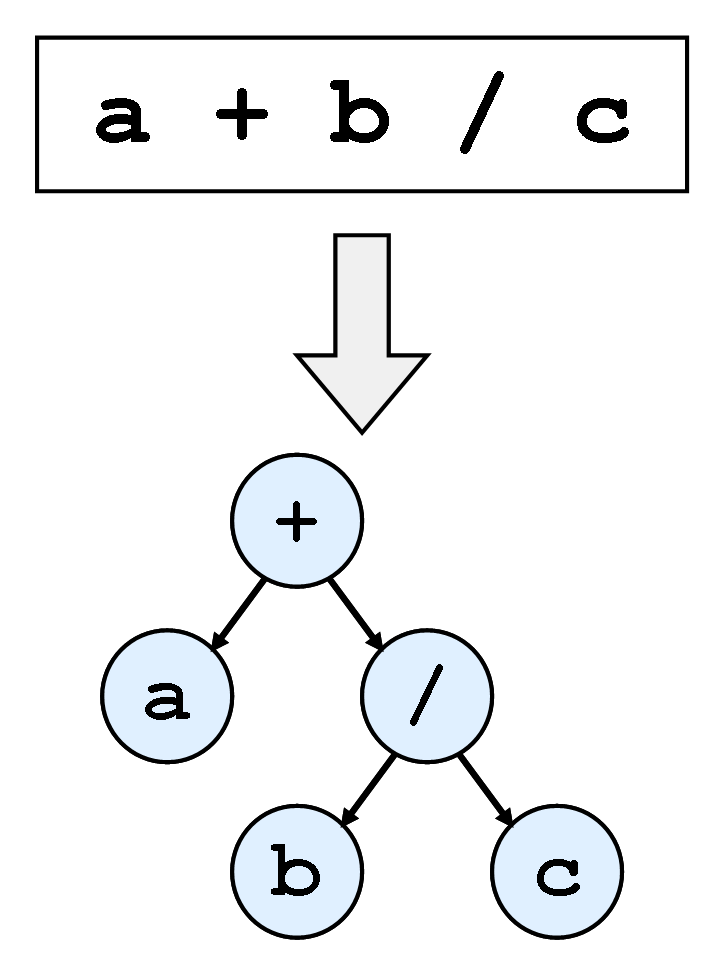
\includegraphics[scale=.4]{recursive-decent.png}
  \caption{递归下降简单示例}\label{fig:recursive-decent}
\end{figure}

通过语法分析,编译器能够完全了解源文件所想表达的含义,从而也就能够生成
{\bf\it 抽象语法树}(AST)。至此,编译器前端的任务就已经完成了,
编译器的后端会根据前端提供的抽象语法树来生成目标代码。
\footnote{因此现在创建一个编程语言变得容易了很多,如rust、swift都是站在了LLVM的肩膀上,
自己负责前端的词法分析和语法分析,将生成代码交给更专业、优化更精细的LLVM。}


\chapter{系统需求分析与总体设计}

% 说明设计原理并进行方案选择
% 阐明为什么要选择这个设计方案(包括各种方案的分析、比较)以及所采用方案的特点

\section{系统需求分析}

% 这部分应该写的是用户需求,明确你做的系统要实现的目标,
% 能处理一些什么样的事务、事务处理流程等。

系统应当具有以下功能:

\begin{itemize}
	\item 识别源代码中的关键字、标识符等
	\item 分析各个语素所组成的语句的语法正确性
	\item 根据源文件生成对应的抽象语法树
	\item 根据抽象语法树生成代码
	\item 对于源文件中出现的错误,能够指出错误类型与位置
\end{itemize}

更具体而言,对于token的分隔应当能适应任何长度、种类的分隔符。
包括但不限于空格符、换行符、制表符等。

对于抽象语法树,应当能够根据节点的层级进行缩进,也应当能够由用户指定
缩进的大小。

在交互方面,应当能正确分析输入的选项,能够指定所编译的源文件,
应当能够指定输出文件,应当能够指定是否输出抽象语法树。

\section{系统总体设计}\label{sec:alldesign}

% 这部分可根据用户需求,设计和规划一个系统,说明清楚系统应该有哪些功能模块,
% 每个模块做什么。最后给出完整的系统模块结构图

\begin{figure}[hbt]
	\centering
	\begin{tikzpicture}
    \node (terminal1) at (0,-0.5) [draw, terminal,
    minimum height=0.5cm] {词法分析器 Lexical Analyzer};

    \node (terminal2) at (0,-2) [draw, terminal,
    minimum height=0.5cm] {语法分析器 Syntax Analyzer};

    \node (terminal3) at (-4,-3.5) [draw, terminal,
    minimum height=0.5cm] {语法树打印器 AST Printer};

    \node (terminal4) at (4,-3.5) [draw, terminal,
    minimum height=0.5cm] {代码生成器 Code Generater};

	\draw[->] (terminal1) --  (terminal2);
	\draw[->] (terminal2) --  (terminal3);
	\draw[->] (terminal2) --  (terminal4);
	\end{tikzpicture}
	\caption{系统模块结构}\label{fig:system_arch}
\end{figure}

系统主要分为四个模块:词法分析、语法分析、打印器和生成器。\autoref{fig:system_arch}
中展示了模块间的关系。

\paragraph{词法分析器} 词法分析器主要负责对源文件进行标记化,区分由
分隔符分隔的标记,并且使用有限自动状态机的方式判断标记的类别(如:{\tt 123}为数字,
{\tt x}为标识符,{\tt int}为关键字),但在这个过程中,并不关心标记之间的关系
\cite{aho1986compilers}(例如:词法分析器能够将括号识别为标记,但并不保证括号是否匹配)。

\paragraph{语法分析器}
语法分析器根据所定义的巴斯克范式对标记序列进行分析并确定其语法结构。
语法分析器使用词法分析器从输入字符流中分离出一个个的“单词”,并将单词流作为其输入,
进行语法检查、并构建由输入的单词组成的抽象语法树\cite{muchnick1997advanced}。

\paragraph{语法树打印器}
语法树打印器负责将生成的抽象语法树形象化地表示出来,主要用于检查系统的正确性。

\paragraph{代码生成器}
代码生成器以语法分析器生成的抽象语法树作为输入,来生成与之向对应的代码,
主要用于检查系统的正确性。

\section{项目架构}

\autoref{tree}中给出了项目的整体架构。
\lstinputlisting[label=tree,caption={项目架构}]{../../project_tree.dat}

\subsection{各文件说明}

{\tt src}文件夹中为主要的源文件,其中,
\begin{itemize}
	\item {\tt next.cc}为词法分析器的实现。
	\item {\tt expr.cc}为语法分析器中分析表达式的部分。
	\item {\tt stmt.cc}为语法分析器中分析语句的部分。
	\item {\tt gen.cc}为语法分析器中生成抽象语法树的部分。
	\item {\tt logger.cc}为代码生成器的实现。
	\item {\tt AST/Logger.cc}为抽象语法树打印器的实现。
\end{itemize}

{\tt include}文件夹中为头文件。

{\tt test}文件夹中为单元测试文件。


\chapter{系统详细设计}

% 指作者对自己的研究工作的详细表述。
% 要求论理正确、论据确凿、逻辑性强、层次分明、表达确切

\section{有关数据结构的定义}

\section{主要算法设计}

% end


\chapter{结果分析}


\chapter{总结与展望}

\section{课程设计总结}

\subsection{工作总结}

整个课程设计从寒假开始,共花费一周时间进行设计,之后花费一周时间完成第一版开发,
再后来的时间进行测试和报告编写,直至\zhtoday{}完成课程设计。

整个项目共有源代码近3000行,报告的源代码有近7000行。详细信息见\autoref{lst:src_count}。

\begin{listing}[hbt]
	\scriptsize
\begin{verbatim}
github.com/AlDanial/cloc v 1.84  T=0.14 s (866.9 files/s, 86345.4 lines/s)
-------------------------------------------------------------------------------
Language                     files          blank        comment           code
-------------------------------------------------------------------------------
TeX                             31            399            160           6766
C++                             42            290            242           2756
C/C++ Header                     9            104             23            452
JSON                             5              0              0            255
Markdown                         3             56              0            158
CMake                           18             46              7            129
YAML                             5              9              6             84
C                                6             13              5             77
make                             1             18              1             50
TypeScript                       1              4              0             39
Bourne Shell                     1              1              0              2
-------------------------------------------------------------------------------
SUM:                           122            940            444          10768
-------------------------------------------------------------------------------
\end{verbatim}
\caption{源代码行数}\label{lst:src_count}
\end{listing}

\subsection{系统的优点}
本次实验中,我成功地完成了任务要求,并且在要求的语法基础上做了许多扩展,
支持了指针类型等C语言常用语法。同时,代码组织结构化,模块分工明确,并且绝大部分
代码都含有注释。

同时,系统还在许多方面做了优化,提高了效率与生成树的质量。

此外,系统很多想法都借鉴与相关操作系统概念,如符号表,数据段等,运行栈等,
可以说和操作系统紧密相连。

\subsection{系统的不足}

系统在语义分析方面还不够完善,并且报错信息也有时不够准确。此外,在设计语法时,
特地选取了适合使用递归下降分析的语法,使得语法解析变得比较简单。
并且系统只支持C语言的一个子集,并不能说是一个完整的C语言编译器前端。

相比于成熟的现代化编译器,我的系统可以说连玩具的算不上,不仅仅在功能上不足,
还在实用性上差距很大,并且运行效率也不高。

\section{工作展望}

完成项目后,我深深地感受到了不足。在今后的学习中,我将进一步探索编译原理有关知识,
尤其是更加理论化的概念与证明,并且将其与操作系统相结合,争取能有一天能够使用
自己创造的语言写一个能编译自身的编译器,并且用它们来创造一个自己的操作系统,
最后把操作系统运行在自己设计的CPU上。

\chapter{体会与感想}

我从听说有编译原理这门课以来,就一直对其充满了好奇。在看到任务的时候,我几乎是
立即决定选择这个任务,实现一个简单的编译器前端。当然,由于编译原理是一个理论性
非常强的分支,因此在初期遇到了巨大的困难。龙书\cite{aho1986compilers}、
虎书\cite{appel2004modern}、鲸书\cite{muchnick1997advanced}我都翻看了,但确实
不能很快理解通透。再后来看了网上但一些例子,自己也试着动手尝试,慢慢地才完成了
整个项目。

从整个项目的完成过程中,我不仅仅在实践中体会编译器及其内部数据结构的运行,
更锻炼了编程的能力和解决问题的能力。

之所以采用了很多操作系统相关概念,是因为我在假期中学习了深入理解计算机系统\cite{bryant2003computer},
其中的很多操作系统思想令我印象深刻。同时我也对把C语言代码变成汇编语言的过程产生
了及其浓厚的兴趣,因为它看起来是如此的繁琐,几乎是不可能完成的任务。

当然,在整个过程中我也意识到了自己的知识的不足,以后也会更刻苦的学习,争取能够
做出自己的编译器。


\backmatter

\begin{ack}
    感谢老师、助教和同学在本次实验中的对我的帮助,特别是许老师和助教许学长,在实验中为我提供了很多建议。
    \par
    在此衷心地对他们表示感谢!
    \par
    特别感谢教材\cite{严蔚敏2002数据结构}与习题册\cite{严蔚敏1998数据结构题集}对我的帮助
\end{ack}

\bibliography{book}

\appendix

\end{document}
\endinput
%%
